\documentclass[twocolumn,superscriptaddress,10pt,showpacs,pra]{revtex4}%
\renewcommand\baselinestretch{1}
\usepackage{mathbbold}
\usepackage{mathrsfs}%
\textheight 260mm

\oddsidemargin=0mm

\topmargin=0in

\renewcommand\baselinestretch{1}


\voffset   -2.75cm

\hoffset  -0.5cm
\usepackage{natbib}
\usepackage{bm}
\usepackage{amsmath}
\usepackage{threeparttable}
\usepackage{amssymb}

\usepackage{amsfonts}

\usepackage[colorlinks,CJKbookmarks,linkcolor=blue]{hyperref}
\usepackage{color}
\usepackage{booktabs}  %���岻ͬ��ϸ�ķָ���
\usepackage{tabularx}  %������
\usepackage{graphicx}%
\renewcommand{\arraystretch}{1.5}
\renewcommand{\textfraction}{0.15}
\renewcommand{\topfraction}{0.85}
\renewcommand{\bottomfraction}{0.65}
\renewcommand{\floatpagefraction}{0.60}
\begin{document}
\title{NMR analog of Bell-type inequalities tests for three qubits}
\author{}
\email{} \affiliation{Department of Modern Physics, University of
Science and Technology of China and Hefei National Laboratory for
Physical Sciences at Microscale, Hefei, Anhui 230026, People's
Republic of China}
\author{}
\email{} \affiliation{Department of Modern Physics, University of
Science and Technology of China and Hefei National Laboratory for
Physical Sciences at Microscale, Hefei, Anhui 230026, People's
Republic of China}
\author{}
\email{} \affiliation{Department of Modern Physics, University of
Science and Technology of China and Hefei National Laboratory for
Physical Sciences at Microscale, Hefei, Anhui 230026, People's
Republic of China}
\author{}
\email{} \affiliation{Department of Modern Physics, University of
Science and Technology of China and Hefei National Laboratory for
Physical Sciences at Microscale, Hefei, Anhui 230026, People's
Republic of China} \affiliation{Fachbereich Physik, Universit\"at
Dortmund, 44221 Dortmund, Germany}
\begin{abstract}
We simulate the violation of MABK inequality for three-qubit GHZ
state in NMR system. Furthermore, we simulate the violation of
different Bell's inequalities for generalized GHZ states in NMR
system, MABK inequality and Chen's inequality. From the experiment,
the results obviously display that MABK inequality is inefficienct
in a region of generalized GHZ states. However, Chen's inequality is
efficienct for any generalized GHZ entangled states.



\end{abstract}

\pacs{03.67.Pp, 03.67.Lx}\maketitle
\subsection*{I. Introduction}
\begin{frame}
 Forty-four years ago, Bell showed that in all local realistic
theories, correlations between the outcomes of measurements in
different parts of a physical system satisfy a certain class of
inequalities \cite{Bell}. However, it is easily found that entangled
states violate these inequalities in quantum mechanics. From this
inequality, the crucial conflict between classical theory and
quantum mechanics was obviously shown. Hence, Bell's work has been
described as "the most profound discovery of science" \cite{Stapp}
or, at least, "one of the greatest discoveries of modern science"
\cite{Zukowski}. After Bell's work, many important generalizations,
including the Clauser-Horne-Shimony-Holt (CHSH) \cite{CHSH} and
Mermin-Ardehali-Belinskii-Klyshko (MABK) inequalities \cite{MABK}
have appeared. A set of multipartite Bell inequalities have been
elegantly derived by Werner and Wolf and by \.{Z}ukowski and Brukner
(WWZB), by using two dichotomic observables per site \cite{WWZB}.
Recently, there has been increasing interest in the subject of
Bell's inequalities, not only to test local realism in quantum
mechanics in a variety of contexts, but also because of their
relation to quantum communication \cite{ Brukner, Brassard, Scarani}
and quantum cryptography \cite{Chen,Acin and Gisin}. For example,
the security of some quantum communication protocols are based on
the loophole-free violation of Bell inequalities \cite{Acin and
Gisin, Barrett, Acin and Brunner}. Furthermore, Bell��s inequalities
can be a useful tool to detect entanglement, which is found to be a
powerful computational resource in quantum computation
\cite{Nielsen}.

In experiments, variety of Bell tests have been performed, starting
with the first experimental tests of Bell inequalities with photons
\cite{Freedman, Aspect, Weihs}. Violation of a Bell inequality has
been observed in a wide range of systems including atoms systems
\cite{Moehring, Matsukevich1, Matsukevich2}, atomic ensembles
\cite{Matsukevich3, Chou}, and trapped ions \cite{Rowe}. Recently,
an experiment to simulate the violation of CHSH inequality has been
carried out in NMR system \cite{Souza}.

In this paper, we simulate the violation of Bell-type inequalities
for three-qubit GHZ state in NMR system. Furthermore, we also
simulate the violation of Bell-type inequalities for generalized GHZ
states in NMR system. Prevenient experiments mainly focused on the
maximal entangled states, such as Bell state, standard GHZ state,
etc. Nonmaximal entangled states were rarely mentioned. The reason
is, such as in photon experiments, preparing a nonmaximal entangled
state is as difficult as standard GHZ state. Scientists may consider
it is not worth the candle in photon system \cite{Lu}. On the other
hand, there are many phenomena disclosed by nonmaximal entangled
states, for instance, the nonmaximal entangled states make lots of
Bell-type inequalities arrive the maximal violation \cite{Acin and
Durt, Methot and Scarani}. There are many open problems about
nonmaximal entangled states. Especially, as the particles and
dimensions increasing, it may exhibit unexpected properties.
Therefore, it is interesting and meaningful to research the
nonmaximal entangled states. We simulate tests for different Bell's
inequalities, MABK inequality \cite{MABK} and Chen's inequality
\cite{k.Chen}in NMR system. From the experiment, the results
obviously display that MABK inequality is inefficient in a region of
generalized GHZ states. However, Chen's inequality is efficient for
any generalized GHZ entangled states. The facts proved that all of
our experimental results are coincident with the prediction of
quantum mechanics.

It is necessary to explain that, in strictly, because NMR qubits are
nuclear spins of atoms bounded together in a single molecule,
separated by a few angstroms. Hence, the situation of an NMR
experiment is inherently local. Our results are also in good
agreement with the local hidden variable theory. It may appear
puzzling that quantum and classical theory are both consistent with
our experiments. However, it can be understood, although the entire
system is local, NMR is only sensible for the deviation part of the
mixed state, which behaves like a "pure entangled state". Hence, our
experiments in NMR system are not really prove the violation of
Bell-type inequalities. This is why we always emphasize that our
experiments are simulation not prove. However, the meaning is that,
when we experimentally simulate the violation of different Bell-type
inequalities for arbitrary generalized three-qubit GHZ states in NMR
system, the results excellently display the theoretical prediction.
It told us, despite of existed many disputes, NMR system may be can
contribute more on some fundamentals of quantum mechanics. After
all, it was less exploited experimentally outside the scope of
optics.  Besides, if our experiment were carried out in a highly
polarized spin ensemble \cite{Anwar}, true entangled states can be
achieved and a contradiction between hidden variables models and
quantum theory could be detected.
\end{frame}
\subsection*{II.Simulation violation of MABK inequality for GHZ state}
\begin{frame}
Let us consider such a scenario: there are three observers Alice
(\emph{A}), Bob (\emph{B}), and Charlie (\emph{C}), each having one
qubit. The formulation of the MABK inequality based on the
assumption that every observer is allowed to choose between two
dichotomic observables. Denote the outcome of observer $X$'s
measurement by $X_{i}, X=A,B,C$, with $i=1,2$. Under the assumption
of local realism, each outcome can either take value $+1$ or $-1$.
In a specific run of the experiment, the correlations between the
measurement outcomes of all three observers can be represented by
the product $A_{i}B_{j}C_{k}$, where $i , j , k=1, 2$. In a local
realistic theory, the correlation function of the measurements
performed by all three observers is the average of $A_{i}B_{j}C_{k}$
over many runs of the experiment,  The MABK inequality reads
\cite{MABK}
%\begin{widetext}%
\begin{eqnarray}\label{MABK}
&|&E(A_{1},B_{2},C_{2})+E(A_{2},B_{1},C_{2})+\nonumber\\
&&E(A_{2},B_{2},C_{1})-E(A_{1},B_{1},C_{1}){}|\leq2.
\end{eqnarray}
%\end{widetext}%
We denote the left-hand side of the MABK inequality by
$\mathcal{B}_{MABK}$ where $-2\leq\mathcal{B}_{MABK}\leq2$. In any
local hidden variable (LHV) theory, the absolute value of a
particular combination of correlations is bounded by 2. However, if
one turns to quantum mechanics, this inequality can be violated. For
MABK inequality, the maximal violation allowed by quantum mechanics
is $4$ \cite{Scarani and Gisin}, which for standard GHZ state,
\begin{equation}\label{standard GHZ state}
\left\vert \Phi \right\rangle=\frac{\sqrt{2}}{2}(\left\vert 000
\right\rangle+\left\vert 111 \right\rangle).
\end{equation}
can be reached by particular observers.

To prepare standard GHZ state from $\left\vert 000 \right\rangle$,
we can use the network as shown in Fig.1, by selecting the rotation
angle $2\theta=\pi/2$. After that, we will measure the spin
projection $\bm{\sigma\cdot n}$, where
$\bm{\sigma}=(\sigma_x,\sigma_y,\sigma_z)$ is the vector form of
Pauli matrices and the two measurement directions for every qubit we
choose here are $\bm{n_1}=(1,0,0)$ and
$\bm{n_2}=(\cos\alpha,\sin\alpha,0)$.

For this special spin projection measurement, the theoretical result
of $\mathcal{B}_{MABK}$ is (for convenience we just ignore the
absolute value sign)
\begin{equation}
\mathcal{B}_{MABK}=3( \cos^{2}\alpha-\sin^{2} \alpha)-1,
\end{equation}
displaying that for $\alpha=0.3041\pi\sim0.6959\pi$ the result
violates MABK inequality and reach the maximal violation value $4$
when $\alpha=\pi/2$, as shown in Fig.4.
\begin{figure} \centering
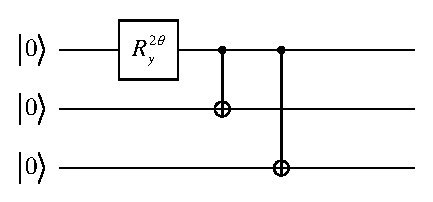
\includegraphics[width=0.8\columnwidth]{net.eps}
\caption{A quantum network for creating a generalize GHZ state. The
initial state is $\left\vert 000 \right\rangle$. After rotating
qubit 1 by the angle $2\theta$ about Y axis, we get
$\cos\theta\left\vert 000 \right\rangle+\sin\theta\left\vert 100
\right\rangle$.Then through two control gates CNOT$_{12}$ and
CNOT$_{13}$, a generalize GHZ state $\cos\theta\left\vert 000
\right\rangle+\sin\theta\left\vert 111 \right\rangle$ will be
created.}
\end{figure}

For experimental implementation using NMR system, there are still
two problems to be solved. Firstly the initial state of NMR at room
temperature is a highly mixed thermal equilibrium state which is
unfit for quantum computation. We can use pseudo-pure state(PPS)
\cite{Gershenfeld} technique to overcome this, that the initial
state is transformed to
\begin{equation}
\rho_{pps}=\frac{(1-\varepsilon)}{2^n}I_{2^n}+\varepsilon\left\vert
\varphi\right\rangle\left\langle\varphi\right\vert,
\end{equation}
which is a mixture of the totally mixed state $I_{2^n}$ unchanged
when applying with unitary transformations and a pure state
$\left\vert \varphi\right\rangle$ which we set to be $\left\vert 0
\right\rangle$ in our experiment with
$\varepsilon=10^{-5}\sim10^{-6}$. So ignoring $I_{2^n}$ which does
not affect NMR experiments and using the entanglement(strictly,
pseudo-entanglement) of the pure part, we can simulate violation of
the Bell-type inequalities we mentioned in this letter. Another
problem is only the spin projection values under computational basis
can be directly measured. The solution is we can rotate the state or
density matrix instead of changing the projective direction,
\begin{eqnarray}
M=Tr(\rho\cdot M_{1})=Tr(\rho\cdot U^{+}M_2U) \nonumber\\
=Tr(U\rho U^{+}\cdot M_2),
\end{eqnarray}
where $M_1$ and $M_2$ is the desired measurement and experimental
measurement, respectively. $U$ is one unitary operation satisfying
$M_1=U^{+}M_2U$. In NMR experiments we can apply $U$ to the density
matrix and then take measurement of $M_2$ equivalent to measuring
$M_1$.

All experiments were performed at room temperature on a Bruker
Avance $400MHz$ NMR spectrometer. In the experiment we used the
spins of three ${}^{13}\!C$ nucle in alanine dissolved in $D_2 O$.
The system Hamiltonian can be written as
\begin{equation}
H_{sys}=\sum_{i=1}^3 \omega_i I_z^i+2\pi\sum_{i<j}^3 J_{ij} I_z^i
I_z^j,
\end{equation}
with the Larmor angular frequencies $\omega_i$ and $J$-coupling
constants $J_{ij}$, whose values are listed in Fig.2.
\begin{figure} \centering
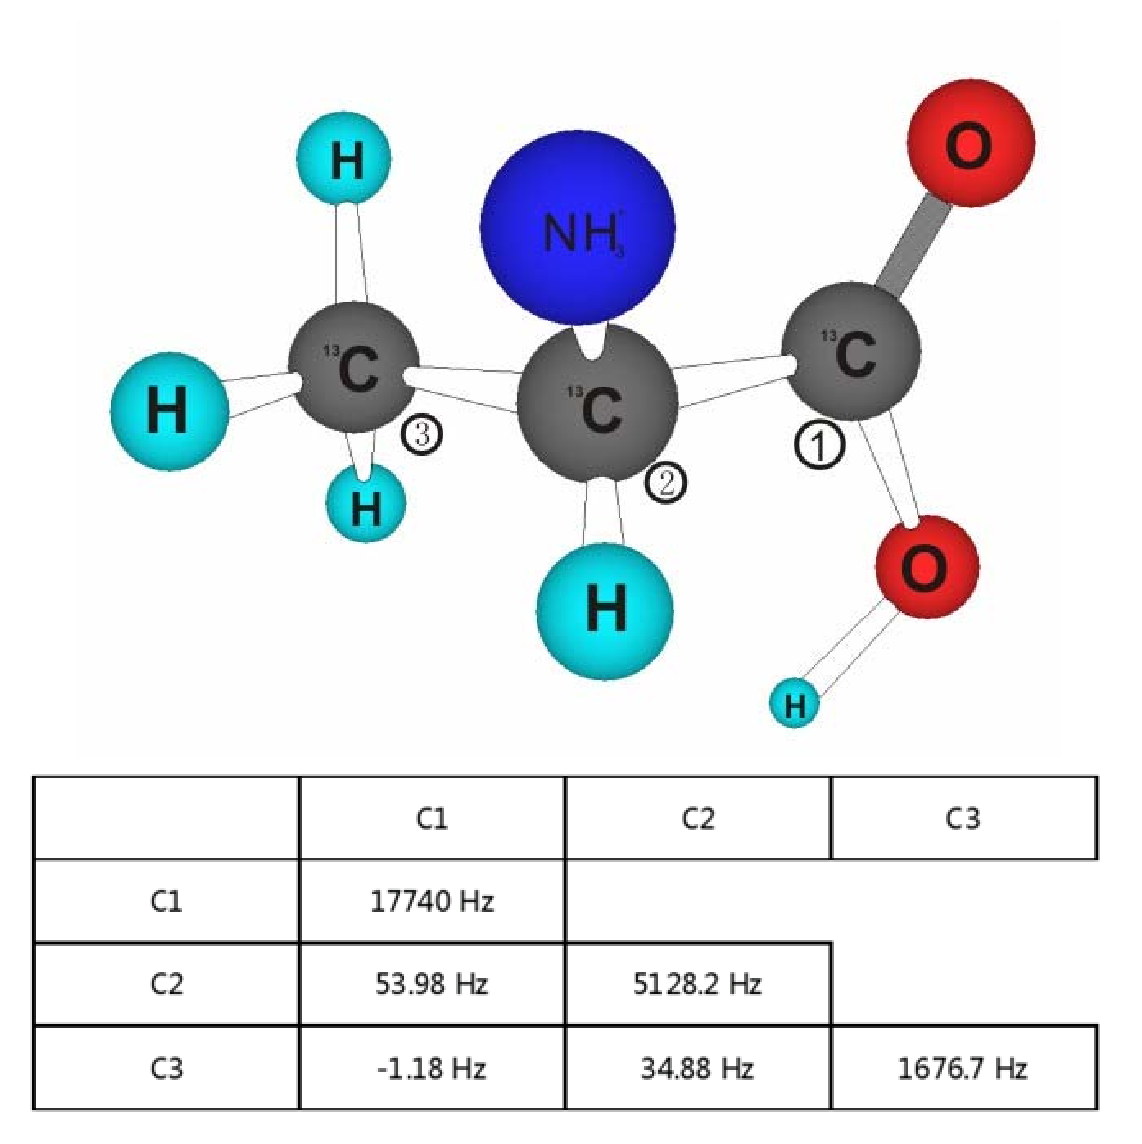
\includegraphics[width=0.8\columnwidth]{structure.eps}
\caption{Molecular structure and Hamiltonian parameters for alanine.
The diagonal elements are the chemical shifts of the three carbon
nuclei and the off-diagonal elements are the J-coupling strengths. }
\end{figure}

The whole experiment was divided into three steps. Firstly, prepare
PPS $\left\vert 000\right\rangle$ from the thermal equilibrium
state, using the spatial average technique \cite{Cory}. Secondly, to
prepare a standard GHZ state, we use a Hardmard gate and two CNOT
gates, that is to say, set $\theta=\pi/2$ in Fig.1. Finally, rotate
the required qubits and execute the projective measurements.

In order to improve the accuracy of radio frequency (RF) pulses, we
use strongly modulating pulse (SMP) techniques \cite{Fortunato} to
simulate the theoretical unitary operations. We also maximize the
effective gate fidelity by averaging over a weighted distribution of
RF field strengths to overcome the inhomogeneity of the RF fields
over the sample. The gate fidelity we calculated for every pulse is
higher than 0.995 considering the RF field inhomogeneity. The range
of the pulse lengths are about from $200\sim 700\mu s$.
\begin{figure} \centering
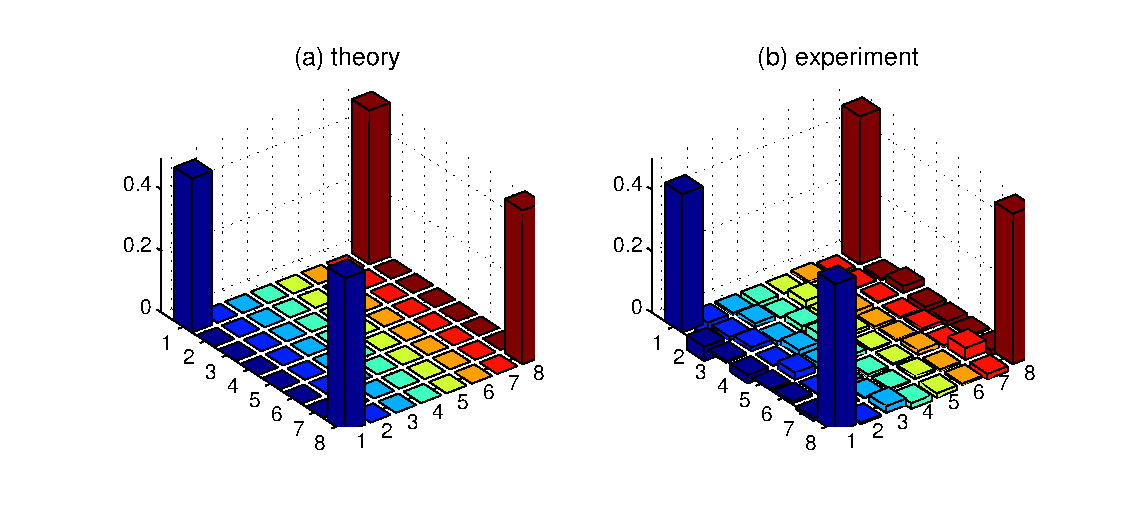
\includegraphics[width=1\columnwidth]{tomo.eps}
\caption{The theoretical (a) and experimental (b) density matrices
of the standard GHZ state $(\left\vert 000 \right\rangle+\left\vert
111 \right\rangle)/{\sqrt{2}}$. The bars' height at the four
vertices of the density matrix is 0.5 theoretically. The fidelity is
0.98.}
\end{figure}

Fig.3 (b) shows a full state tomography of the standard GHZ state in
experiment. The overall fidelity is
\begin{equation}
F=\frac{Tr(\rho_{th}\rho_{exp})}{\sqrt{(Tr(\rho^2_{th})Tr(\rho^2_{exp}))}}=0.98,
\end{equation}
We take several sets of observers to do the corresponding measure on
standard GHZ state. The result is shown in the Fig.4, which the blue
squares stand for the experiment results, and the red thick line
stands for the theoretical result. Clearly, the experiment result is
in excellent agreement with the theoretical expectation in quantum
mechanics.

Of course, if we had considered the huge mixed state $I_{2^n}$ into
the experiment, we would get the result in agreement with the
classical theory. Therefore, this is why we emphasize that the
experiments are simulation not proof.
\begin{figure} \centering
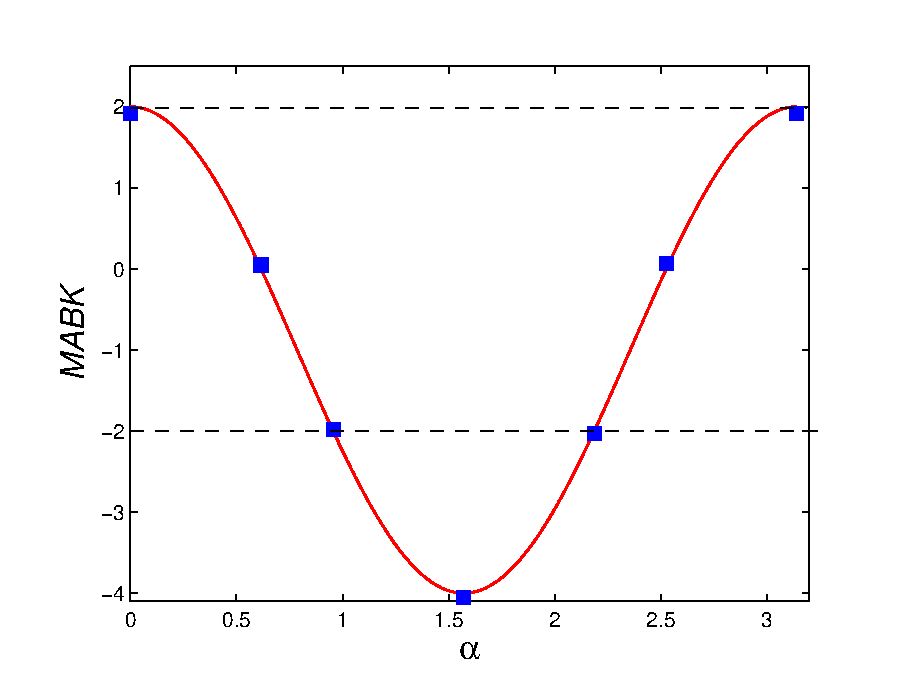
\includegraphics[width=0.8\columnwidth]{MABK1.eps}
\caption{The values of $\mathcal{B}_{MABK}$ as a function of
$\alpha$. The red thick line stands for the theoretical result, and
the blue square stands for the experiment result.}
\end{figure}
\end{frame}
\subsection*{III. Simulation violation of MABK inequality for generalize GHZ states}
\begin{frame}
So far, almost all prevenient Bell experiments were focus on maximal
entangled states, such as Bell state and standard GHZ state.
Recently, sorts of unexpected properties about nonmaximal entangled
states have been shown\cite{Acin and Durt, Methot and Scarani}.
Therefore, we simulate the violation of MABK inequalities for
generalized GHZ states in NMR system further. The generalized GHZ
states can be expressed as
\begin{equation}\label{generalized GHZ state}
\left\vert \Psi \right\rangle=\cos\theta\left\vert 000
\right\rangle+\sin \theta\left\vert 111 \right\rangle.
\end{equation}
which $\theta\in[0, \frac{\pi}{2}]$.

In this experiment, we choose the directions of the two measurements
for every particles are $\bm{n_1}=(1,0,0)$ and $\bm{n_2}=(0,1,0)$.
For these special spin projection measurements, the theoretical
result of $\mathcal{B}_{MABK}$ for generalized GHZ states satisfies
such a function,
\begin{equation}
|\mathcal{B}_{MABK}|=|-4\sin(2\theta)|.
\end{equation}
From the function above, it is shown that the maximal violation is
obtained when $\theta=\frac{\pi}{4}$ just the standard GHZ state.
Obviously, the MABK inequality only in the region of
$\theta\in[\frac{\pi}{12}, \frac{5\pi}{12}]$ is efficient, in other
words, only in such region the inequality can be violated.
Therefore, MABK inequality is not efficient in the whole region of
generalized GHZ states.

We measured a set of generalized GHZ states with particular angle
$\theta$ in the experiment.
 The result is shown in Fig.5, which the blue
squares stand for the experiment results, and the red thick line
stands for the theoretical result. The experiment result is
coincident with prediction of quantum theory.

\begin{figure}
\begin{center}
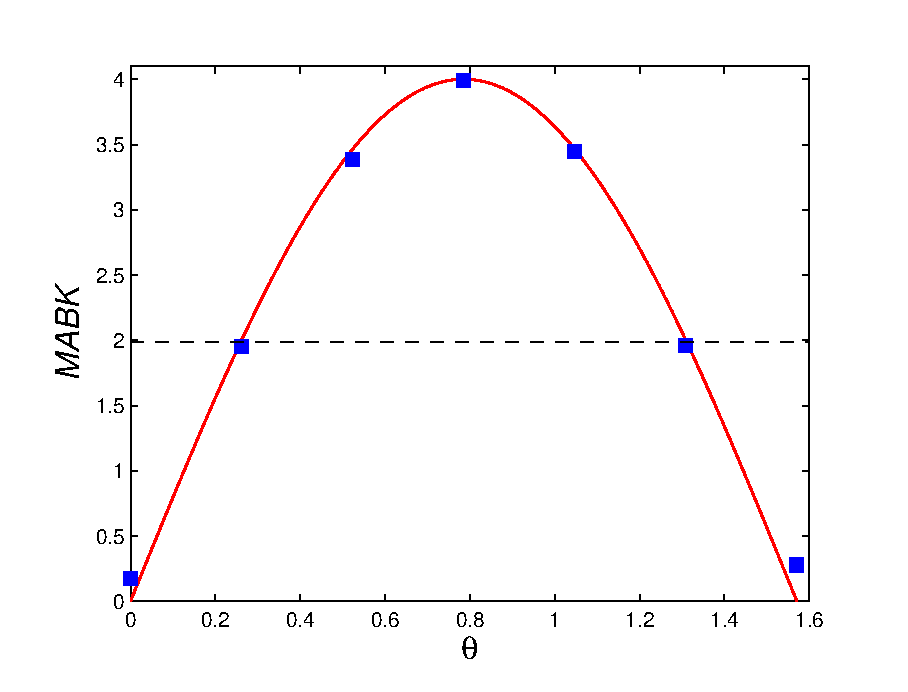
\includegraphics[width=0.40\textwidth]{MABK2.eps}
\caption{The values of $\mathcal{B}_{MABK}$ as a function of
$\theta$. The red thick line stands for the theoretical result, and
the blue square stands for the experiment result.}
\end{center}
\end{figure}
\end{frame}
\subsection*{IV. Simulation violation of Chen's inequality for generalize GHZ states}
\begin{frame}

In Section {III}, the experiment results display that MABK
inequality is not efficient in the whole region of generalized GHZ
states. However, this phenomenon already has been found several
years in theory. Scarani and Gisin \cite{Scarani and Gisin} firstly
found that there exist pure states of three qubits that do not
violate the MABK inequality. These states are just the generalized
GHZ states \eqref{generalized GHZ state}. It is shown that for
$\theta\leq \pi/12$ or $\theta\geq5\pi/12$ the states
\eqref{generalized GHZ state} do not violate the three-qubit MABK
inequality. Hence, Scarani and Gisin deduced that MABK inequalities
and more generally the family of Bell's inequalities with two
observables per qubit, may not be the 'natural' generalizations of
the CHSH inequality to more than two qubits \cite{Scarani and
Gisin}. whereafter, a set of multipartite Bell inequalities has been
elegantly derived, which is the WWZB inequality \cite{WWZB}.
Actually, The WWZB inequalities include MABK inequalities as special
cases. Furthermore, \.{Z}ukowski \emph{et.al} proved and showed that
\cite{Zukowski and Brukner and Laskowski and Wiesniak} (i)for
$N=even$, although the generalized GHZ state does not violate MABK
inequalities, it violates the WWZB inequality, and (ii) for $N=odd$
and $sin(2\theta)\leq1/\sqrt{2^{N-1}}$, the correlations between
measurements on qubits in the generalized GHZ state satisfy all Bell
inequalities for correlation functions, which involve two dichotomic
observables per local measurement station.

As to obtain such a Bell-type inequality involving only two
measurement settings per observer, which is violated by the
generalized GHZ state in the whole region of $\theta$ for any number
of qubits, several notable work were shown. Chen and Wu \emph{et
al.} developed several Bell inequalities in terms of both
probabilities and correlation functions for three qubits, which can
be seen numerically to be violated by any pure entangled state
\cite{J. L. Chen, C. F. Wu}. Recently, a more significant progress
derived by K. Chen \emph{et al.} \cite{k.Chen}. They presented a
family of Bell inequalities involving only two measurement settings
of each observer for $N>2$ qubits, which is not only violated by the
$N$-qubit generalized GHZ state in the whole region,but also the
amount of maximal violation grows exponentially as $2^{(N-2)/2}$.

From the above description in theory, more efficient Bell-type
inequalities for generalized GHZ states are derived. However, no
experiments aim to display it so far. We simulate the violation of
Chen's inequality for generalized GHZ states. On the other hand, we
simulate or predict results for different Bell-type inequality tests
in NMR system.

For three-qubit system, Chen's inequality can be written as

%\begin{widetext}%
\begin{eqnarray}
\mathcal{B}_{Chen}=\frac{1}{2}(E(A_{1},B_{1},C_{1})+E(A_{1},B_{2},C_{1})+E(A_{2},B_{1},C_{1})-\\[-4pt]
E(A_{2},B_{2},C_{1})+E(A_{1},B_{1},C_{2})+E(A_{1},B_{2},C_{2})+\\
E(A_{2},B_{1},C_{2})-E(A_{2},B_{2},C_{2}))+E(C_{1})-E(C_{2}),
\end{eqnarray}
%\end{widetext}%
which $|\mathcal{B}_{Chen}|\leq2$ in the LHV model.

In experiment, based on [29], we take the directions of two
measurement about $A$ and $B$ as $\bm{n_1}=(1,0,0)$ and
$\bm{n_2}=(0,1,0)$. For $C$, the directions of two measurement are
$\bm{n_1}=(\sin\alpha\cos(-\frac{\pi}{4}),\sin\alpha\sin(-\frac{\pi}{4}),\cos\alpha)$
and
$\bm{n_2}=(\sin(\pi-\alpha)\cos(-\frac{\pi}{4}),\sin(\pi-\alpha)\sin(-\frac{\pi}{4}),\cos(\pi-\alpha))$,
where
\begin{eqnarray}
\alpha=\tan^{-1}(\sqrt{2}\tan(2\theta)),\quad\quad\quad\quad
   0\leq\theta\leq\frac{\pi}{4}\nonumber
\\\alpha=\tan^{-1}(\sqrt{2}\tan(2\theta))+\pi,\quad\quad
   \frac{\pi}{4}\leq\theta\leq\frac{\pi}{2}
\end{eqnarray}
Then, we can get the values of $\mathcal{B}_{Chen}$ as a function of
$\theta$,
\begin{equation}
\mathcal{B}_{Chen}=2(2\sin^{2}(2\theta)+\cos^{2}(2\theta))^{1/2}.
\end{equation}
 The results are always larger than $2$ no matter what values $\theta$ take. It means that, the
 whole region of generalized GHZ states can violate the inequality by a set of suitable observation angles.

 Obviously, Chen's
 inequality is more efficient than MABK inequality for generalized
 GHZ states. The experimental result is shown in the Fig.6, which perfectly simulate
 the violation of Chen's inequality for generalize GHZ states. It is
 shown that our experimental result is in good agreement with
 quantum mechanical
 theory.

\begin{figure} \centering
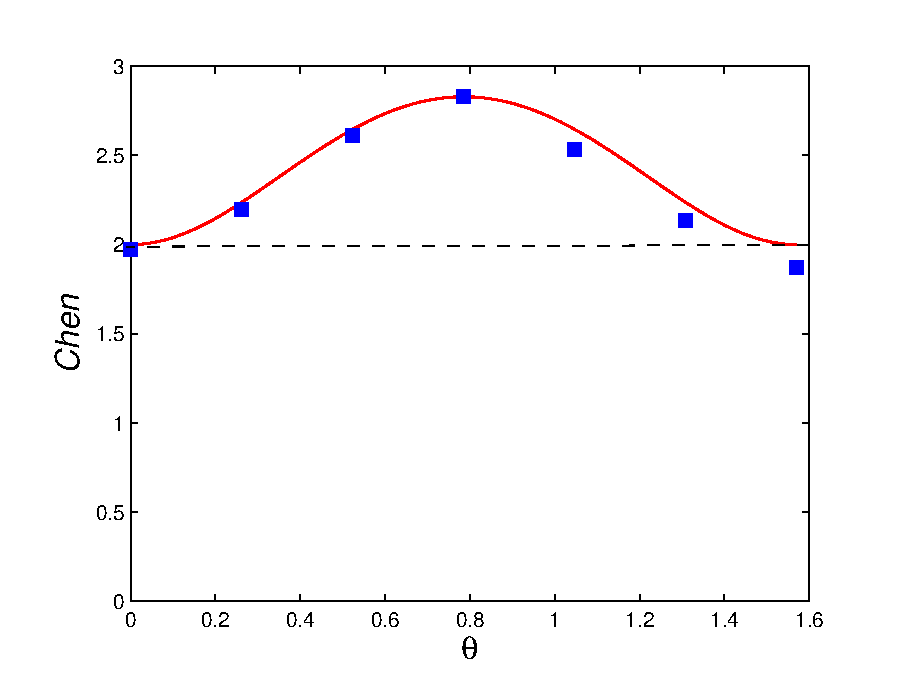
\includegraphics[width=0.40\textwidth]{Chen.eps}
\caption{The values of $\mathcal{B}_{Chen}$ as a function of
$\theta$. The red thick line stands for the theoretical result, and
the blue square stands for the experiment result.}
\end{figure}

\end{frame}
\subsection*{V. Conclusions}
\begin{frame}
In summary, we simulate the violation of MABK inequalities for
three-qubit GHZ state in NMR system. Furthermore, we focus on the
nonmaximal entangled states, the violation of MABK inequality for
generalized states in NMR system are shown. The data of experiments
are exactly coincident to the result of quantum theory. As to
exhibit test of different Bell-type inequality for generalized GHZ
states, we also simulate Chen's inequality in NMR system. Compared
the result of Chen's inequality with that of MABK inequality, it is
obviously display that MABK inequality is not efficient in whole
region of generalized GHZ state.However, Chen's inequality is
efficiency for any generalized GHZ entangled states. As a refined
tool and technique for experimentally realizing quantum computation
in the last decade, NMR still contributes to many fundamental
problems of quantum mechanics now. In the future, we will still pay
attention to this area.
\end{frame}

\subsection*{Acknowledgments}
\begin{frame}
The authors are grateful to Ya Wa, Ping Zou and Jing Zhu for their
help and interesting comments and discussions. Financial support
comes from National Natural Science Foundation of China, the CAS,
Ministry of Education of PRC, and the National Fundamental Research
Program. It is also supported by Marie Curie Action program of the
European Union.
\end{frame}


















\begin{thebibliography}{99}

\bibitem{14} J. F. Du, P. Zou, M. J. Shi, L. C. Kwek, J. W. Pan, C. H. Oh, A. Ekert, Daniel K. L. Oi, and M. Ericsson (2003) Observation of geometric phases for mixed states using NMR interferometry, Phys. Rev.
Lett. 91, 100403.
\bibitem{15} M. Ericsson, D. Achilles, J. T. Barreiro, D. Branning, N. A. Peters, and P. G.
Kwiat (2005) Measurement of geometric phase for mixed states using
single photon interferometry, Phys. Rev. Lett. 94, 050401.
\bibitem{16} D. G. Cory, M. D. Price, and T. F. Havel (1998) Nuclear magnetic resonance spectroscopy: an experimentally accessible paradigm for quantum
computing, Physica D: Nonlinear Phenomena 120, 82.
\bibitem{17} E. M. Fortunato, M. A. Pravia, N. Boulant, G. Teklemariam, T. F. Havel and D. G. Cory (2002) Design of strongly modulating pulses to implement precise effective Hamiltonians for quantum information processing,
J. Chem. Phys. 116 (17), 7599.
\bibitem{18} M. A. Pravia, N. Boulant and J. Emerson (2003) Robust control of quantum information, J. Chem. Phys. 119, 9993.
\bibitem{19}  T. S. Mahesh and D. Suter (2006) Quantum-information processing using strongly dipolar coupled nuclear spins, Phys. Rev. A. 74,
062312.
\bibitem{20} A. Carollo, I. Fuentes-Guridi, M. F. Santos, and V. Vedral (2003) Geometric phase in open systems, Phys.
Rev. Lett. 90, 160402.
\bibitem{21} D. M. Tong, E. Sj\"{o}qvist, L. C. Kwek, and C. H. Oh (2004) Kinematic approach to the mixed state geometric phase in nonunitary evolution, Phys. Rev. Lett. 93, 080405.
\bibitem{22} M. Ericsson, A. K. Pati, E. Sj\"{o}qvist, J. Br\"{a}nnlund, and D. K. L. Oi (2003) Mixed state geometric phases, entangled systems, and local unitary transformations, Phys. Rev. Lett. 91, 090405.
\bibitem{23} D. Suter, K. T. Mueller, and A. Pines (1988) Study of the Aharonov-Anandan quantum phase by NMR interferometry, Phys. Rev. Lett. 60, 1218.


\end{thebibliography}

\end{document}
